\documentclass{article}
\usepackage{graphicx} % Required for inserting images
\usepackage[margin=1in]{geometry}
\usepackage{amsmath,amsthm,amssymb, graphicx, multicol, array, enumitem}
\usepackage{commath, bm, siunitx, mathtools}
\usepackage[colorlinks=true,urlcolor=blue,linkcolor=blue,citecolor=red,pdfencoding=auto,psdextra]{hyperref}
\usepackage{physics}
\usepackage{listings}
\usepackage{subcaption}


\title{Implementation of the Projected Variational Quantum Dynamics Algorithm}
\author{G. Adam Cox, I-Tung Chen, Sanskriti Joshi, Tommy Nguyen}
\date{February 28, 2023}

\begin{document}

\maketitle

\section{Introduction}
Quantum simulations are a fundamental way to understand quantum phenomena. Researchers try to understand quantum phenomena experimentally by building up systems with qubits and letting their system evolve according to given constraints and variables. However, systems with many degrees of freedom are hard to create experiments for due to the vast space of variables that need to be controlled. This is why simulating quantum systems on computers is a very powerful tool if it can be done correctly and efficiently. Additionally, since quantum systems are inherently "quantum", it is believed that these systems are best simulated on a quantum computer as they have the nature of being quantum themselves and therefore might be easier to simulate by leveraging this quantumness (entanglement, coherence, etc.). In QHACK, we probe this idea by studying quantum simulations, but more specifically, the time dynamics of quantum systems as governed by the Schrodinger equation on quantum computers:
\begin{equation}\label{schro}
    \frac{i \partial\ket{\Psi}}{\partial t} = \hat{H} \ket{\Psi}
\end{equation}
We stick to time-independent hamiltonians H as this is the easier case out of the two, albeit still NP-hard :), and this gives the solution:
\begin{equation}\label{timeevo}
    \ket{\Psi(t)} = e^{-i\hat{H}t}\ket{\Psi(0}
\end{equation}
As referenced in this Nature paper two months ago \cite{nature_2021}, the problem of trying to implement the above equation is very tricky due to H being almost anything you want and is a huge problem for \textbf{quantum computing today}! There are two main approaches to tackle this problem: variational and decomposition techniques which each have many subfields within them. We will not give an overview of the different methods as the Nature paper does this already, but we instead focus on a specifc algorithm within the variational umbrella: the projected variational quantum dynamics algorithm (pVQD) as discovered by Stefano Barison a year ago \cite{Barison_2021}. The novel idea of this algorithm is that it evolves variational parameters by optimizing them at each time step to resemble a small Trotter step using gradient descent. And so this leverages \textbf{hybrid classical-quantum computing} techniques for efficient computation. Stefano has shown that pVQD is an improvement over the time-dependent variational algorithm \cite{PhysRevX.7.021050} by being global: updating all parameters at once, and has linear scaling with respect to the number of parameters. However, in \cite{Barison_2021}, pVQD has only been used for quantum simulations on a spin chain system and hasn't been tested on actual quantum hardware. In this hackathon, we attempt a couple of novel approaches which has been divided into the following sections below:
\begin{enumerate}
    \item Reproduce the results found in the figures in \cite{Barison_2021} with qiskit and test the reproducibility.
    \item Code the pVQD algorithm with Pennylane's quantum language which is suited for quantum machine learning applications. Since pVQD has a gradient descent step, we believe that Pennylane's built-in functionality to incorporate machine learning techniques will improve the efficiency of this algorithm for actual runtime on a quantum simulator and qpu.
    \item Run the algorithm on an actual quantum hardware device: IBM's 7 qubit Nairobi machine, and compare it to the previous simulations above.
\end{enumerate}

\section{Short Background to pVQD}
This section has been added here for coherence throughout this paper. A more detailed description of the algorithm should be looked at in \cite{Barison_2021}. Here we just go over the main ideas.
\subsection{pVQD Algorithm}
Our goal is to simulate eq.\ref{timeevo}. We do this by starting with a parameterized ansatz state $\ket{\psi_{w(t)}} = \prod_d \prod_i R^{i,d}_\sigma (w_i(t))\ket{\psi_0}$ where $w(t) \in \mathbb{R}^p$ is a vector of p parameters describing our state at each time t for each ith qubit. $R_\sigma$ is a rotation around the axis $\sigma$ and d is the depth of the circuit (how many times its gets repeated). After each trotter step $\delta t$, our time evolved state is:
\begin{equation}
    \ket{\phi(t+\delta t)} = e^{-i\hat{H}\delta t}\ket{\psi_{w(t)}}
\end{equation}
The pVQD aims to maximize:
\begin{equation}
    argmax_{dw} \ \ |\bra{\phi(t+\delta t)}\ket{\psi_{w+dw}} |^2
\end{equation}
by finding a dw that does this. This is done through a gradient descent step:
\begin{equation}
    dw^{new} = dw^{old} - \eta \nabla_{dw} L(dw^{old}, \delta t)
\end{equation}
where L is the cost function we aim to minimize which describes the step in-fidelity:
\begin{equation}
    L(dw, \delta t) = \frac{1-|\bra{\phi(t+\delta t)}\ket{\psi_{w+dw}} |^2}{\delta t^2}
\end{equation}
where $\eta$ is the typical learning rate in ML.

\subsection{Model}
The model that we simulate is the transverse ising field model as the one done in the paper:
\begin{equation}
    H = J\Sigma_{i=1}^{N} \sigma^z_i \sigma^z_{i+1} + h\Sigma_{i=1}^{N} \sigma^x_i
\end{equation}
where we use N = 3 qubits, J = 1/4, h=1.
\section{Implementation with Qiskit \cite{Barison_2021}}
\begin{figure}[!htb]
    \centering
        \includegraphics[width=4in]{Figure_2.png}
        \caption{Average infidelity $\Delta_F$ over the number of samples over the entire time duration with 60 steps and a depth of 3. }
        \label{fig1}
\end{figure}
\begin{figure}[!htb]
        \centering
        \includegraphics[width=4in]{Figure_3.png}
        \caption{Magnetization measured on qubit 0 with varying amount of shots. (Top) $\sigma_x$ (Bottom) $\sigma_z$ }
        \label{fig2}
\end{figure}
 The source code that \cite{Barison_2021} uses can be found here: \hyperlink{https://github.com/StefanoBarison/p-VQD}{https://github.com/StefanoBarison/p-VQD} while our adaptation of this code in qiskit can be found here: \hyperlink{https://github.com/NnguyenHTommy/p-VQD}{https://github.com/NnguyenHTommy/p-VQD}. We reproduce Fig.2 and Fig.3 found in \cite{Barison_2021} with our own Fig.\ref{fig1} and Fig.\ref{fig2}. Fig.\ref{fig1} is a plot of the total infidelity between our simulated pVQD state and the exact state over all time steps. We don't know how the exact state was computed but we were given the exact state at each time step from the github. We see that as we increase the number of samples (shots), the average infidelity decreases which makes sense because our statistics are better. However, we see that we don't really get an improvement until we transition from $10^6$ to $10^7$ samples. This is in contrast to Fig. 2 in their paper which we believe is because we only took one measurement at each amount of samples while they took 10 measurements. Additionally, comparing the two figures, our order of magnitude for the infidelity is 10x lower suggesting that our revised method of calculating the infidelity is better.
 \newline \newline
 Next looking at Fig.\ref{fig2}, we can see that as we increase the number of shots, we get closer and closer to the exact results for the magnetization. In fact, already at 8000 shots, the pVQD algorithm does surprisingly well. This is in contrast to the TDVA algorithim which needs 80,000 shots to get results that look like they fit to the exact results \cite{PhysRevX.7.021050}. Our results are consistent with Fig.3 in \cite{Barison_2021} so we know that we are implementing things correctly in qiskit, yet we also run with more varying amount of shots than they did to see how bad/good we can get. We see that with 80 shots, pVQD doesn't give accurate results while  80,000 shots is not much better than 8000 shots. This seems to indicate a scaling + saturation law with the number of shots. One thing to also note is that the pVQD algorithm seems to simulate $\sigma_z$ better than $\sigma_x$. We think this is because we apply $R_x$ and $R_y$ rotations for our circuit ansatz and so this would lead to some variance in $\sigma_x$ but not $\sigma_z$. Here we see that 8000 shots are needed for a pretty accurate representation of the exact state and from\cite{Barison_2021}, the pVQD algorithm needs 10x less shots to do this giving more justification that pVQD is better.

\section{Implementation with Pennylane}

We implemented the pVQD algorithm using Xanadu's open-source quantum machine learning library, `pennylane` for an open-chain Transverse Field Ising Model consisting of three qubits,

\begin{equation}
    H = J\Sigma_{i=0}^{2} \sigma^z_i \sigma^z_{i+1} + h\Sigma_{i=0}^{2} \sigma^x_i
\end{equation}

for $J = 0.25$ and $h = 1$. We chose this specific system in order to make direct comparison to the previously published work\cite{Barison_2021}.

Implementation of the pVQD algorithm consisted of four components: defining the Hamiltonian, defining our circuit model, defining our cost function, then implementing the optimization loop over our time-span. Our total time span, $T$, lasted 2.0, with step sizes, $\delta t$ of 0.05. (Time units are arbitrary.)  Our code repository is found here: \url{https://github.com/gadamc/uw_qx_pvqd_qhack2023}. Relevant files are 'circuit.py', 'vqd.py', and 'test-vqd.ipynb'.

Our Hamiltonian implementation used `pennylane`'s built-in Hamiltonian function with appropriate coefficients

\begin{lstlisting}[language=Python]
import pennylane as qml

def hamiltonian(coupling_strength=0.25, field_strength=1):
    coefficients = [field_strength]*3
    coefficients += [coupling_strength]*2

    obs = [qml.PauliX(0), qml.PauliX(1), qml.PauliX(2),
           qml.PauliZ(0) @ qml.PauliZ(1),
           qml.PauliZ(1) @ qml.PauliZ(2)]

    return qml.Hamiltonian(coefficients, obs)
\end{lstlisting}

To apply the Hamiltonian to our state in the algorithm, we utilized the `pennylane` function `ApproxTimeEvolution` with a single time step, $\delta t$.

Our multilayered circuit, $C(w)$ consisted of a combination of individual qubit rotations about X or Y (alternating at each layer, $l$) and IsingZZ rotations for the coupled qubits. This is of the form

\begin{equation}
    C(w) = \Pi_l \Pi_i R_{\alpha}^{(i)} (w_{i,l}) \Pi_j e^{-i w_{j,l} \sigma^z_j \sigma^z_{j+1}}
\end{equation}

where $\alpha$ is either $x$ or $y$, alternating between layers, $l$.

This circuit can be found here \url{https://github.com/gadamc/uw_qx_pvqd_qhack2023/blob/main/circuit.py#L15} and is visualized in Fig. \ref{circuit}.

\begin{figure*}[!htb]
    \centering
        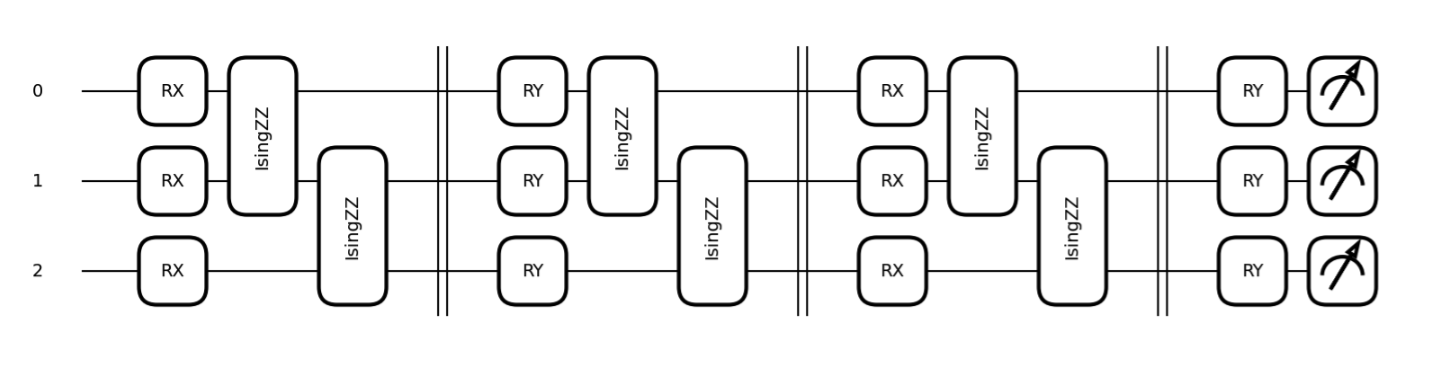
\includegraphics[width=5in]{circuit.png}
        \caption{Circuit ansatze for three-qubit Transverse Ising Model with three layers.}
        \label{circuit}
\end{figure*}

Our cost function for this work was the \emph{infidelity} between state $\phi(w, \delta t)$ and and  $\psi(w + dw)$

\begin{equation}
    L = 1 - |\bra{\phi(w,\delta t)} \ket{\psi(w + dw}|^2
\end{equation}

This differs, slightly, from the previous work as we did not normalize by our time step, $\delta t^2$. However, given that $\delta t$ is a constant throughout, the final optimized parameters should be the same.

At each time step between 0 and $T$ we optimized our parameters using the standard pennylane `GradientDescentOptimizer` with a step size of 0.1. For each time step, approximately 40 to 60 optimization steps were needed to converge (Fig.\,\ref{opt_v_time}).

\section{Results}


The primary benefit of the original work was to show that pVQD outperforms TVDA as measured by the cumulative infidelity of the optimized circuits for different number of circuit shots. Because we simulated with an exact state vector simulator, our cumulative infidelity is independent of circuit shots and a direct comparison cannot be made at this time.

\subsection{Observables}

Next we show the results of observables obtained running on different hardware, compared to the "exact" solution. We note that the exact solution provide here was reproduced from data found in the original work. We have not verified the accuracy of the "exact" solution shown here. We have measured the average magnetization along both the $x$ and $z$ directions using the pennylane state vector simulator (Figs.\,\ref{default.qubit.sigma_x},\ref{default.qubit.sigma_z}), IBM's QASM simulator (Figs.\,\ref{ibmq_qasm.sigma_x},\ref{ibmq_qasm.sigma_z} ) and IBM's Nairobi QPU (Figs.\,\ref{ibm_nairobi.sigma_x},\ref{ibm_nairobi.sigma_z}).

Utilizing the optimized circuit parameters at each time step, we run the circuit on different hardware and measure our observables. The Jupyter notebook 'run-fit-params-to-get-observables.ipynb' was used to run our optimized circuit on real hardware.

\begin{figure*}[!htb]
    \centering
        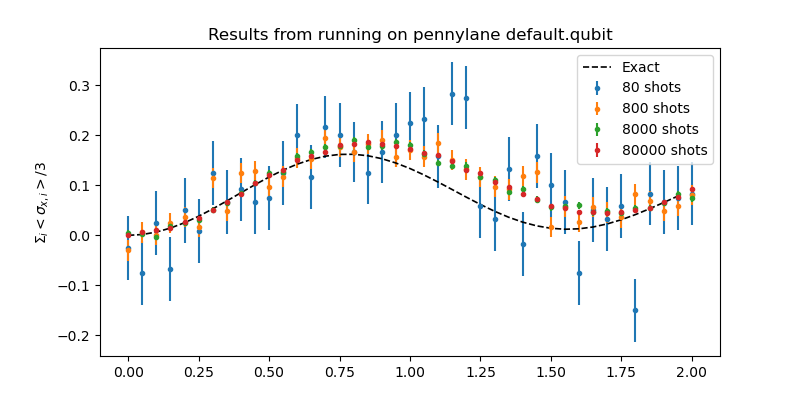
\includegraphics[width=5in]{sigma_x_default.qubit.png}
        \caption{Average magnetization of the three qubits along the direction of the applied magnetic field ($x$ direction). These data were simulated with the pennylane state vector simulator.}
        \label{default.qubit.sigma_x}
\end{figure*}

\begin{figure*}[!htb]
    \centering
        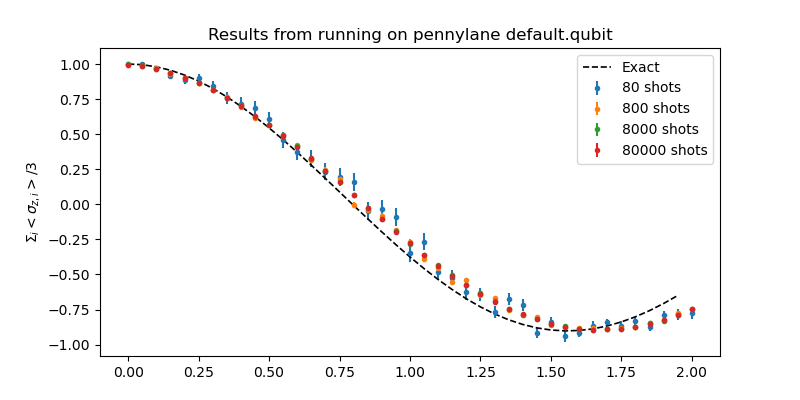
\includegraphics[width=5in]{sigma_z_default.qubit.png}
        \caption{Average magnetization of the three qubits along the $z$ direction. These data were simulated with the pennylane state vector simulator.}
        \label{default.qubit.sigma_z}
\end{figure*}

\begin{figure*}[!htb]
    \centering
        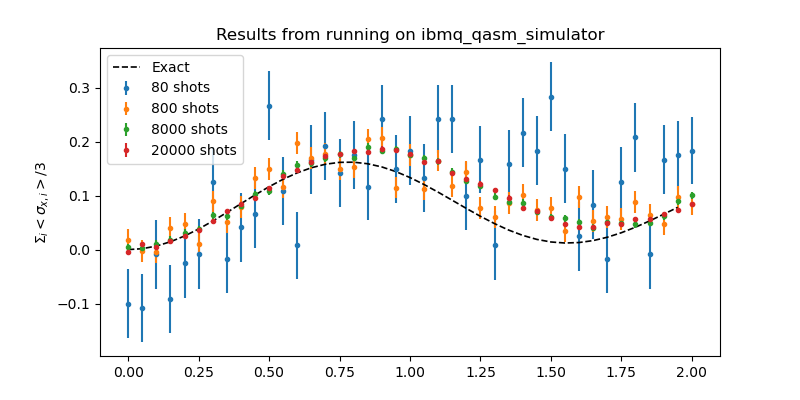
\includegraphics[width=5in]{sigma_x_ibmq_qasm_simulator.png}
        \caption{Average magnetization of the three qubits along the direction of the applied magnetic field ($x$ direction). These data were simulated with the IBM QASM simulator.}
        \label{ibmq_qasm.sigma_x}
\end{figure*}

\begin{figure*}[!htb]
    \centering
        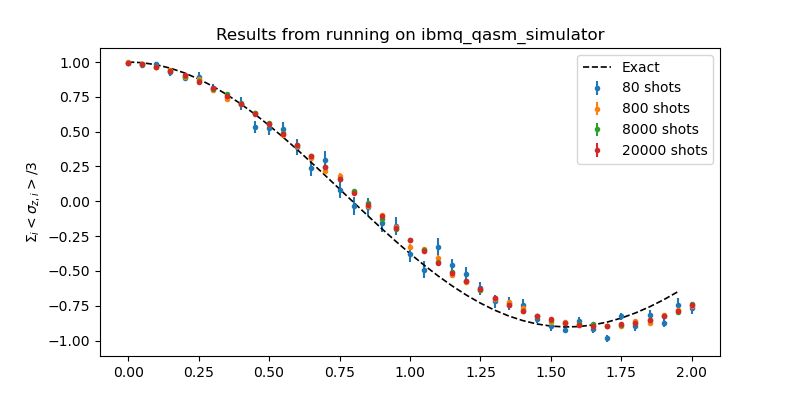
\includegraphics[width=5in]{sigma_z_ibmq_qasm_simulator.png}
        \caption{Average magnetization of the three qubits along the $z$ direction. These data were simulated with the IBM QASM simulator.}
        \label{ibmq_qasm.sigma_z}
\end{figure*}


\begin{figure*}[!htb]
    \centering
        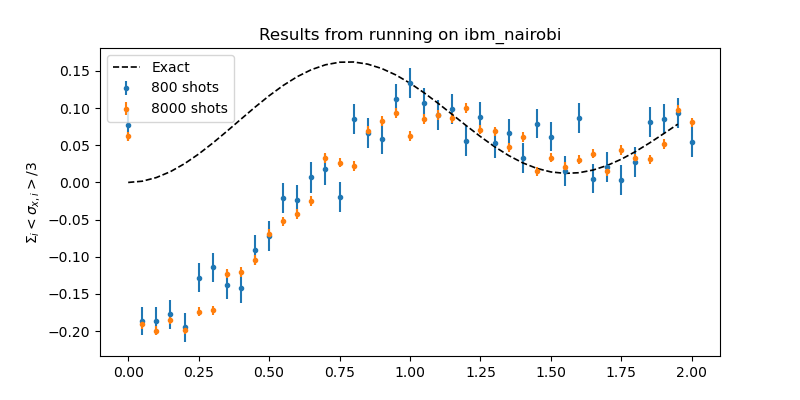
\includegraphics[width=5in]{sigma_x_ibm_nairobi.png}
        \caption{Average magnetization of the three qubits along the direction of the applied magnetic field ($x$ direction). These data were measured with the IBM Nairobi QPU.}
        \label{ibm_nairobi.sigma_x}
\end{figure*}

\begin{figure*}[!htb]
    \centering
        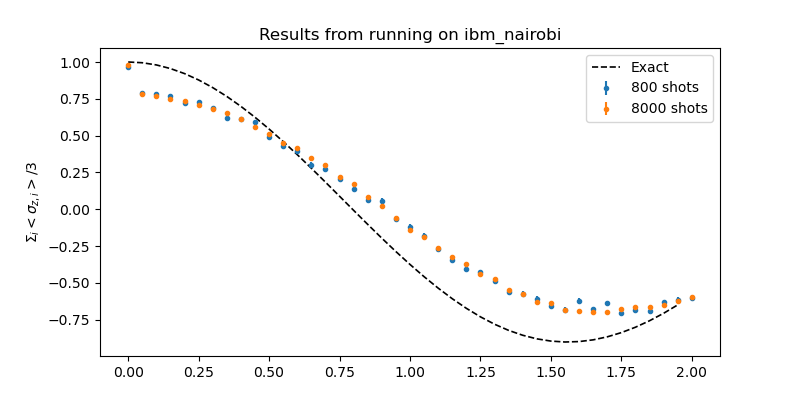
\includegraphics[width=5in]{sigma_z_ibm_nairobi.png}
        \caption{Average magnetization of the three qubits along the  $z$ direction. These data were measured on the IBM Nairobi QPU.}
        \label{ibm_nairobi.sigma_z}
\end{figure*}

\subsection{Optimization Steps}

Next, for comparison to the original work, we show the number of optimization steps required for each time step. Because the pennylane state vector simulator exactly simulates the quantum state the number of optimization steps when using the simulator is independent of the number of shots (Fig.\,\ref{opt_v_time}).

\begin{figure*}[!htb]
    \centering
        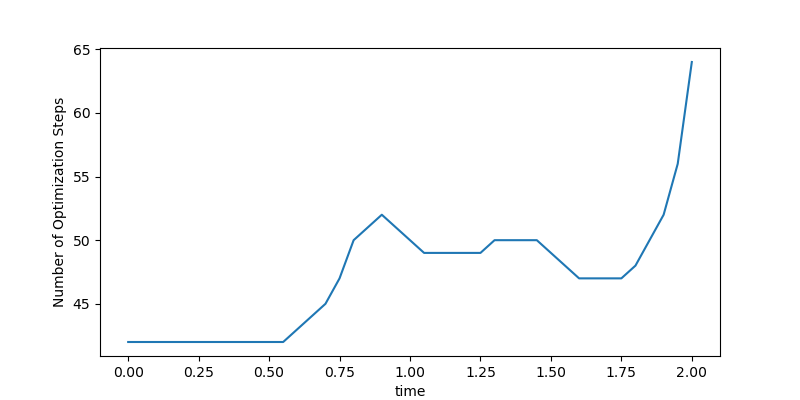
\includegraphics[width=5in]{optimization_steps_v_time_default.qubit.png}
        \caption{Number of optimization steps required at each time-step of the simulation.}
        \label{opt_v_time}
\end{figure*}

We also observed the infidelity for each step of the optimization routine at two different points in time of the simulation, $t = 0.05$ and $t = 2.0$, (Figs.\,\ref{infidel_v_step_0.05}, \ref{infidel_v_step_2.0})

\begin{figure*}[!htb]
    \centering
        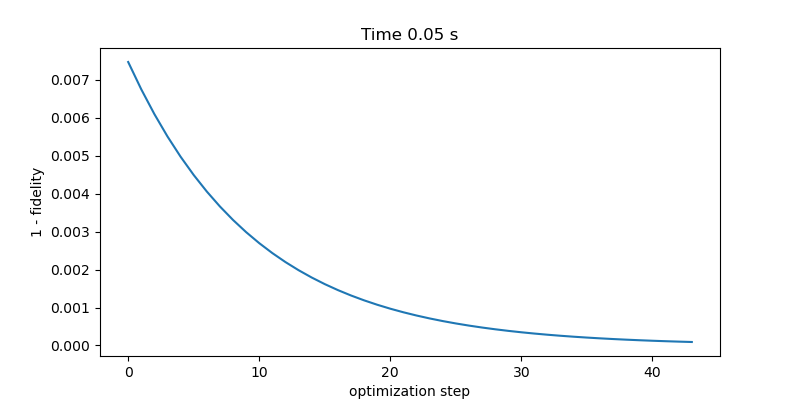
\includegraphics[width=5in]{cost_function_v_step_t0.05.png}
        \caption{State infidelity at each optimization step at t = 0.05.}
        \label{infidel_v_step_0.05}
\end{figure*}


\begin{figure*}[!htb]
    \centering
        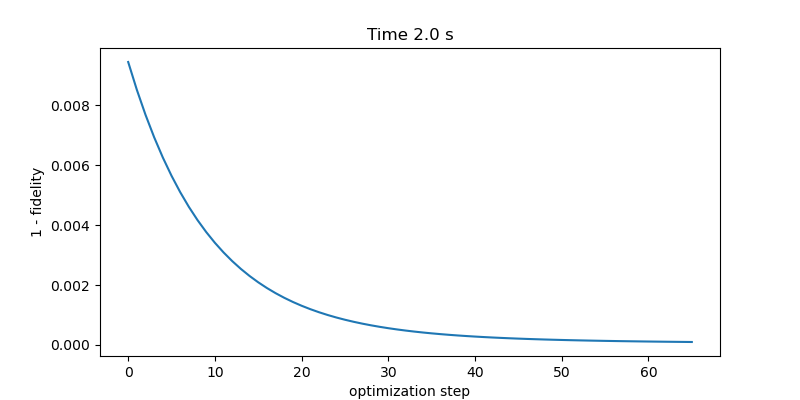
\includegraphics[width=5in]{cost_function_v_step_t2.0.png}
        \caption{State infidelity at each optimization step at t = 2.0.}
        \label{infidel_v_step_2.0}
\end{figure*}

While we have utilized a slightly different optimization function, the number of steps required to optimize the circuit is comparable to the original work. Future work on this project will likely include the implementation of the exact costs functions implemented in \cite{Barison_2021}.


\section{Discussion}
Here we have also shown how pennylane facilitates research of this kind with it's built-in tools. This can be clearly seen comparing the code base used here to the original work. Looking at Figs.\,\ref{default.qubit.sigma_x},\ref{default.qubit.sigma_z} we see that our pennylane simulations models the behavior as in the qiskit version Fig.\ref{fig2} i.e. as we increase the amount of shots, the curves get closer and closer to the exact solution. This shows that our pennylane version is working as intended and we implemented it correctly. However, one thing to note is that even if we increase the amount of shots  to 80,000, the curve doesn't simulate the exact solution completely. There is always a difference as seen in Figs.\,\ref{default.qubit.sigma_x},\ref{default.qubit.sigma_z} between times t =1  and t = 1.75. We believe this might be because of the way we simulated with an exact state vector and a future direction would be to try and implement the local and global operators as described in \cite{Barison_2021}. On the flip side, because we implemented the exact state vector directly in pennylane, the time it takes to simulate is reduced by $\sim 100x$ which is a huge improvement! We think this is because of pennylane's efficiency in doing gradient descent rather than qiskit having to import outside ML methods and incorporate them in the code. Now looking at Figs.\,\ref{ibmq_qasm.sigma_x},\ref{ibmq_qasm.sigma_z} where we run on IBM's simulator that is supposed to model IBM's qpus with noise, we see that the curves are farther away from the exact curve as compared to Figs.\,\ref{default.qubit.sigma_x},\ref{default.qubit.sigma_z}. This is likely due to the noise introduced in the IBM simulator. Finally, we run our pennylane code on IBM's Nairobi machine qpus and this is given in Figs.\,\ref{ibm_nairobi.sigma_x},\ref{ibm_nairobi.sigma_z}. Based on the results of Figs.\,\ref{ibm_nairobi.sigma_x},\ref{ibm_nairobi.sigma_z}, the limitations of simulating the evolution of quantum systems appear to be the errors in the actual QPUs that were available. We find that actual quantum computer are very noisy and the pVQD algorithm doesn't give a good fit in comparison the actual result. We also see that the magnetization at the final time step seems to correspond quite nicely to the exact solution so we think there might be some solution bias in this algorithm. A follow-up would be try error mitigation techniques in combination with our pennylane pVQD algorithm.

Another interesting observation is the number of optimization steps required as a function of time (Fig.\,\ref{opt_v_time}). At larger absolute time values, $t ~ 2.0$, the number of optimization steps required to minimize the cost function begins to increase. Although there are not enough data to draw conclusions, the increase in the last few time steps appears to increase at a much higher (exponential?) rate. Does this imply, that the state of the system is beginning to change much more rapidly over time, requiring more gradient descent steps to find our new optimal circuit parameters? It's not clear to us that this is the case.  At large time values, the change in the total x- and z-components of the qubit spin states are comparable to the change found at earlier times.

\subsection{Future Work}
Oh man. There are so many future directions in which this work can lead into but we didn't have the time to implement everything we wanted to since this is indeed a hackathon! Additionally, while we were working through this project, more and more ideas kept popping up! Here is a list of possible future directions:
\begin{enumerate}
    \item In respect to the quantum chemistry challenge at QHACK, we can try to simulate the Be$H_2$ molecule and perform time dynamic simulations of the molecule under external electromagnetic fields.
    \item Try other various gradient descent ML schemes with applications to this algorithm to see if we can improve on it.
    \item Randomized benchmarking on the average error of pVQD circuits. In a way pVQD is very similar to randomized benchmarking due to way of choosing the circuit ansatz. Since there are in total 24 clifford group operators, perhaps randomized operators for the ansatz might give a better result?
    \item Optimize circuit parameters based on the SWAP test, and other figures of merit.
    \item Vary the circuit ansatz that they use and see what kind of ansatz would work best for pVQD
\end{enumerate}

\bibliography{ref}
\bibliographystyle{plain}
\end{document}
